%GiG
\documentclass{beamer} 
\usetheme{Copenhagen}
\setbeamertemplate{navigation symbols}{}
\setbeamertemplate{headline}{}
\DeclareMathOperator*{\argmax}{arg\,max}

\usepackage{hyperref}


\definecolor{azure}{rgb}{0.0, 0.5, 1.0}
%\newcommand{\tblue}[1]{\textcolor{blue}{#1}}
\newcommand{\tblue}[1]{{\Large {\textcolor{azure}{#1}}}}
\newcommand{\thblue}[1]{{\Huge {\textcolor{azure}{#1}}}}
\newcommand{\hred}[1]{{\textcolor{red}{#1}}}
\newcommand{\furl}[1]{{\footnote{\url{#1}}}}

\newcommand{\mypause}{\pause}
%\newcommand{\mypause}{}

\title[Saravanan Thirumuruganathan] 
{Lecture 9: Naive Bayes, SVM, Kernels}

\author[CSE 5334, Data Mining] 
{Instructor: Saravanan Thirumuruganathan}

\date[] 

\begin{document}


\begin{frame}
  \titlepage
\end{frame}

%\begin{frame}{Outline}
%  \tableofcontents
%  % You might wish to add the option [pausesections]
%\end{frame}

\section{Outline}

\begin{frame}
\frametitle {Outline}
    \begin{enumerate}
        \item Probability basics
        \item Probabilistic Interpretation of Classification
        \item Bayesian Classifiers, Naive Bayes
        \item Support Vector Machines
    \end{enumerate}
\end{frame}


%\begin{frame}{In-Class Quizzes}
%\begin{itemize}
%\item {\Large {\bf URL:}} {\LARGE \bf \url{http://m.socrative.com/}} 
%\item {\Large {\bf Room Name:} {\LARGE \bf 4f2bb99e}}
%\end{itemize}
%\end{frame}


\section{Probabilistic Interpretation of Classification}
\begin{frame}{} 
    \begin{center}
        \thblue{Probability Basics}
    \end{center}
\end{frame}


\begin{frame}{Sample Space}
    \begin{itemize}
        \item {\bf Sample Space:} A space of events that we assign probabilities to
        \item Events can be binary, multi-valued, or continuous
        \item Events are mutually exclusive
        \item Examples:
        \begin{itemize}
            \item Coin flip: \{head, tail\}
            \item Die roll: \{1,2,3,4,5,6\}
            \item English words: a dictionary
            \item Temperature: $\mathbb{R}_{+}$ (Kelvin)
        \end{itemize}
    \end{itemize}
\end{frame}

\begin{frame}{Random Variable}
    \begin{itemize}
        \item A variable, $X$, whose domain is the sample space, and whose value is somewhat uncertain
        \item Examples:
        \begin{itemize}
            \item $X$ = coin flip outcome
            \item $X$ = first word in tomorrow's headline news
            \item $X$ = tomorrow's temperature 
        \end{itemize}
    \end{itemize}
\end{frame}

\begin{frame}{Probability for Discrete Events}
    \begin{itemize}
        \item Probability $P(X=a)$ is the fraction of times $x$ takes value $a$
        \item Often we write it as P(a)
        \item Examples:
        \begin{itemize}
            \item Fair Coin: P(head)=P(tail)=0.5
            \item Slightly Biased Coin: P(head)=0.51, P(tail)=0.49
            \item Two Face's Coin: P(head)=1, P(tail)=0
            \item Fair Dice: P(getting 1 in a die roll) = 1/6
        \end{itemize}
    \end{itemize}
\end{frame}

\begin{frame}{Probability for Discrete Events}
    \begin{itemize}
        \item P(A=``head or tail in a fair coin'') $$0.5 + 0.5 = 1$$
        \item P(A=``even number in a fair dice roll'') $$1/6 + 1/6 + 1/6 = 0.5$$
        \item P(A=``two dice rolls sum to 2 in a fair dice'') $$1/6 * 1/6 = 1/36$$
    \end{itemize}
\end{frame}

\begin{frame}{Axioms of Probability}
    \begin{center}
        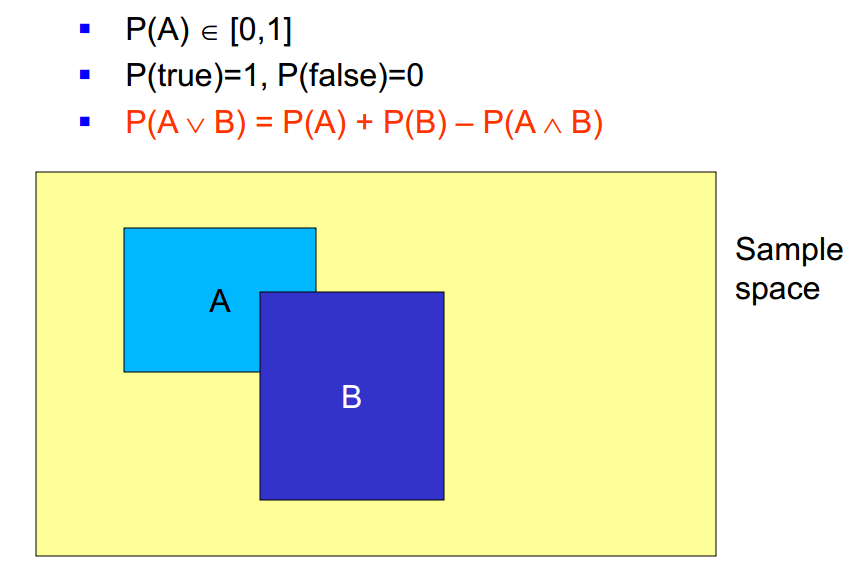
\includegraphics[scale=0.3]{axiomsOfProbability.png}
    \end{center}
\end{frame}

\begin{frame}{Simple Corollaries}
    \begin{itemize}
        \item $P(A') = 1 - P(A)$
        \item If $A$ can take $k$ different values $a_1, \ldots, a_k$, $$P(A=a_1) + \ldots + P(A=a_k) = 1$$
        \item {\bf Law of Total Probability:} 
        \begin{itemize}
            \item $P(A) = P(A \cap B) + P(A \cap B')$
            \item $P(A) = \sum_{i=1}^{k} P(A \cap B=b_i)$ if $B$ takes $k$ values $b_1, \ldots, b_k$
        \end{itemize}
    \end{itemize}
\end{frame}

\begin{frame}{Law of Total Probability\furl{http://people.reed.edu/~jones/Courses/P02.pdf}}
    \begin{center}
        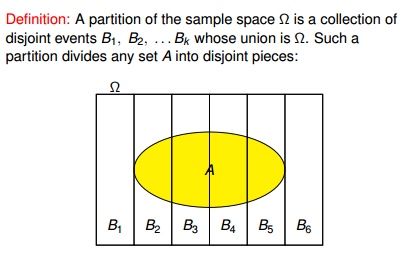
\includegraphics[scale=0.6]{lawOfTotalProbability.png}
    \end{center}
\end{frame}

\begin{frame}{Probability Table}
    \begin{center}
        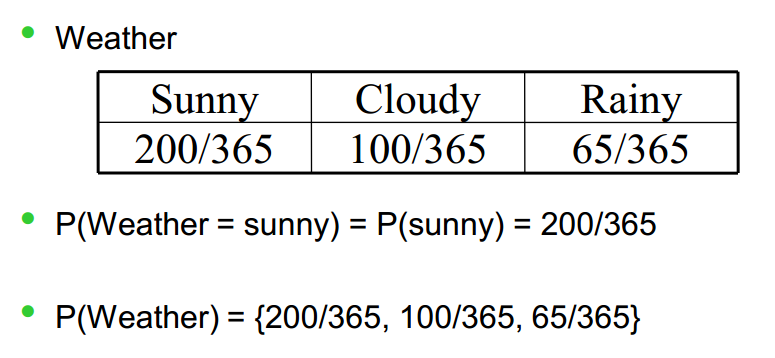
\includegraphics[scale=0.3]{probTbl.png}
    \end{center}
\end{frame}
\begin{frame}{Joint Probability Table}
    \begin{center}
        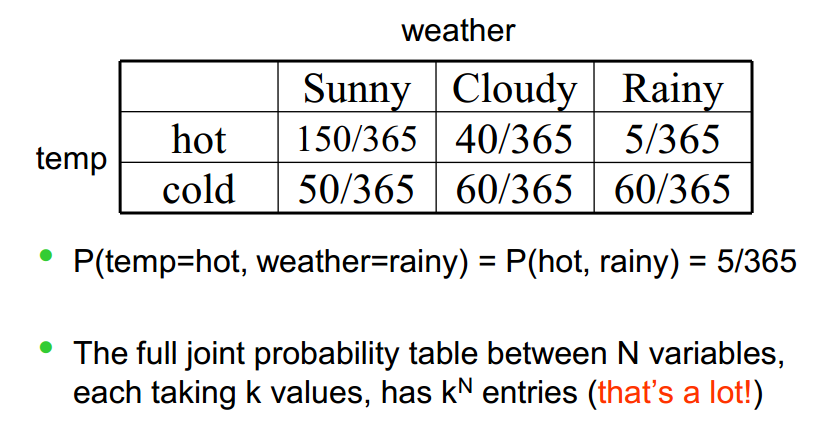
\includegraphics[scale=0.3]{jointProbTbl.png}
    \end{center}
\end{frame}
\begin{frame}{Marginal Probability Table}
    \begin{center}
        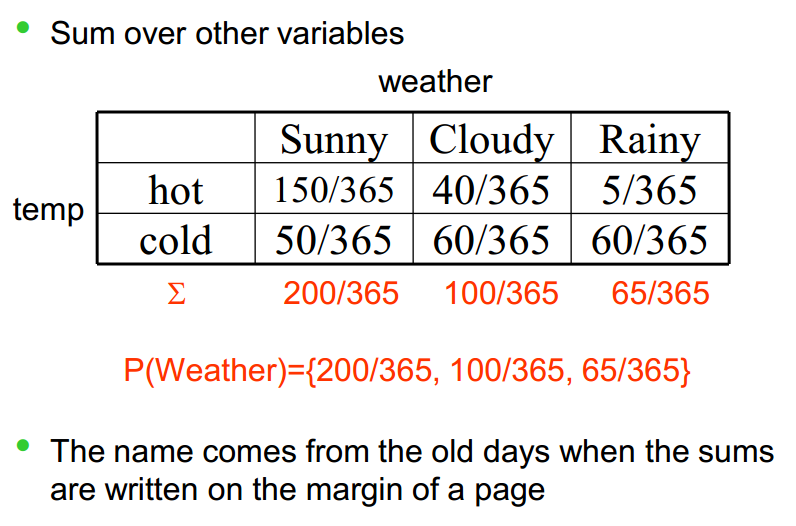
\includegraphics[scale=0.3]{marginalProbTbl1.png}
    \end{center}
\end{frame}
\begin{frame}{Marginal Probability Table}
    \begin{center}
        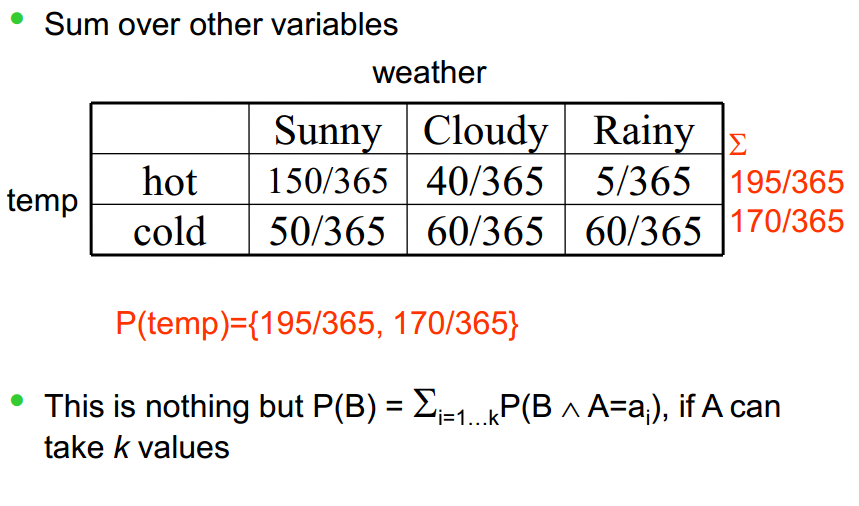
\includegraphics[scale=0.3]{marginalProbTbl2.png}
    \end{center}
\end{frame}

\begin{frame}{Conditional Probability}
    \begin{itemize}
        \item $P(A=a|B=b)$ = fraction of times when random variable $A$ took a value of $a$, within the region where random variable $B=b$
    \end{itemize}
    \begin{center}
        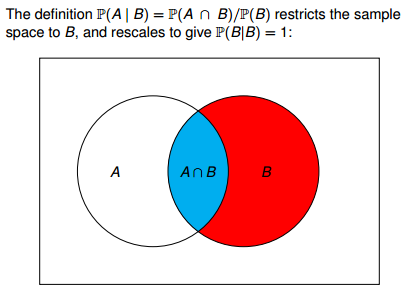
\includegraphics[scale=0.5]{condnlProb.png}
    \end{center}
\end{frame}

\begin{frame}{Conditional Probability}
    \begin{itemize}
        \item Consider a roll of a fair dice
        \item $A$: it rolled $1$. $P(A) = 1/6$ 
        \item $B$: it rolled an odd number. $P(B) = 3/6 = 0.5$
        \item Suppose, I knew that $B$ happened. What is the probability that $A$ happened? \pause
        \item $$P(A|B) = \frac{P(A \cap B)}{P(B)} = \frac{1/6}{1/2} = \frac{1}{3}$$
    \end{itemize}
\end{frame}

\begin{frame}{Conditional Probability}
    \begin{itemize}
        \item {\bf Conditional Probability:} $P(A|B) = \frac{P(A \cap B)}{P(B)}$
        \item {\bf Multiplication Rule:} $P(A \cap B) = P(A|B) P(B)$
        \item {\bf Chain Rule:}
            \begin{itemize}
                \item $P(A_1, A_2) = P(A_1) P(A_2|A_1)$
                \item 
                    \begin{align*}
                        P(A_1, A_2, A_3) &= P(A_3|A_1,A_2) P(A_1,A_2) \\ 
                                         &= P(A_3|A_1,A_2) P(A_2|A_1) P(A_1)
                    \end{align*}
                \item 
                    \begin{align*}
                        P(A_1, A_2, A_3) &= P(A_1|A_2,A_3) P(A_2,A_3) \\
                                         &= P(A_1|A_2,A_3) P(A_2|A_3) P(A_3)
                    \end{align*}
                \item $P\left(\cap_{i=1}^{k} A_i \right) = \prod_{i=1}^{k} P\left( A_i | \cap_{j=1}^{i-1} A_j \right)$
            \end{itemize}
    \end{itemize}
\end{frame}

\begin{frame}{Bayes Theorem}
    \begin{itemize}
        \item $P(A|B) = \frac{P(A \cap B)}{P(B})$
        \item $P(B|A) = \frac{P(A \cap B)}{P(A})$
        \item Proof of Bayes Theorem:
            \begin{align*}
                P(A \cap B) &= P(A|B) P(B) \\ 
                            &= P(B|A) P(A) \\
                P(A|B) P(B) &= P(B|A) P(A) \\
                P(A|B)      &= \frac{P(B|A) P(A)}{P(B)}
            \end{align*}
    \end{itemize}
\end{frame}

\begin{frame}{Independence}
    \begin{itemize}
        \item Two events A, B are independent, if (all 3 definitions are equivalent)
        \begin{itemize}
            \item $P(A \cap B) = P(A) P(B)$
            \item $P(A|B) = P(A)$
            \item $P(B|A) = P(B)$
        \end{itemize}
    \end{itemize}
\end{frame}

\begin{frame}{Independence Misused}
    \begin{center}
        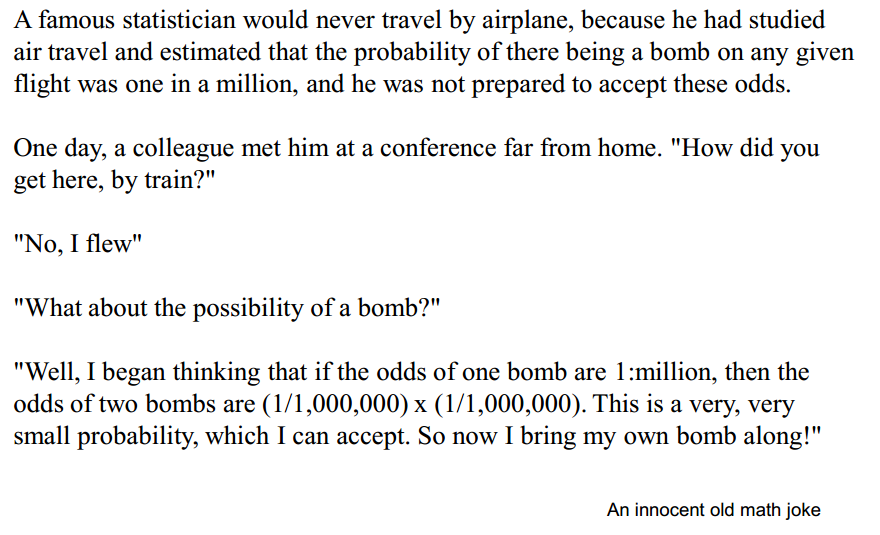
\includegraphics[scale=0.36]{independenceJoke.png}
    \end{center}
\end{frame}

\begin{frame}{Independence}
    \begin{itemize}
        \item Independence between random variables is typically obtained via domain knowledge
        \item Suppose $A$ and $B$ be two independent random variables that can take $k$ different values $a_1, \ldots, a_k$ and $b_1, \ldots, b_k$
        \item The joint probability table typically has $k^2$ parameters
        \item If random variables are independent, then only $2k-2$ parameters
        \begin{itemize}
            \item $k=2$, $4$ vs $2$
            \item $k=10$, $100$ vs $18$
            \item $k=100$, $10,000$ vs $198$
        \end{itemize}
        \item This is something great for data mining!
    \end{itemize}
\end{frame}

\begin{frame}{Conditional Independence}
    \begin{itemize}
        \item Random variables can be dependent, but {\bf conditionally independent}
        \item Your house has an alarm
        \begin{itemize}
            \item Neighbor John will call when he hears the alarm
            \item Neighbor Mary will call when she hears the alarm
            \item Assume John and Mary don‟t talk to each other
        \end{itemize}
        \item JohnCall independent of MaryCall? \pause
        \begin{itemize}
            \item No - If John called, likely the alarm went off, which increases the probability of Mary calling
            \item $P(MaryCall | JohnCall) \neq  P(MaryCall)$
        \end{itemize}
    \end{itemize}
\end{frame}

\begin{frame}{Conditional Independence}
    \begin{itemize}
        \item If we know the status of the alarm, JohnCall won't affect Mary at all
        \item $P(MaryCall | Alarm, JohnCall) = P(MaryCall | Alarm)$
        \item We say JohnCall and MaryCall are {\bf conditionally independent}, given Alarm
        \item In general A, B are conditionally independent given C
        \begin{itemize}
            \item $P(A | B, C) = P(A | C)$ or
            \item $P(B | A, C) = P(B | C)$ or 
            \item $P(A, B | C) = P(A | C) * P(B | C)$
        \end{itemize}
    \end{itemize}
\end{frame}

\begin{frame}{} 
    \begin{center}
        \thblue{Probabilistic Interpretation of Classification}
    \end{center}
\end{frame}

\begin{frame}{Probabilistic Classifiers}
    \begin{itemize}
        \item Type of classifiers that, given an input, produces a {\em probability distribution} over a set of classes 
        \begin{itemize}
            \item Probability that this email is spam is X and not spam is Y
            \item Probability that this person has tumour is X and no tumour is Y
            \item Probability that this digit is $0$ is X, $1$ is Y, $\ldots$
        \end{itemize}
        \item Most state of the art classifiers are probabilistic
        \item Even $k$-NN and Decision trees have probabilistic interpretations
    \end{itemize}
\end{frame}


\begin{frame}{Prior Probability}
    \begin{itemize}
        \item $P(A)$: Prior or unconditional probability of $A$
        \item Your belief in $A$ in the absence of additional information
        \item Uninformative priors
        \begin{itemize}
            \item Principle of indifference: Assign equal probabilities to all possibilities
            \item Coin toss, P(head)=P(tail)=$1/2$
        \end{itemize}
        \item Often you get from domain knowledge or from data 
        \item P(email is spam) = $0.8$
    \end{itemize}
\end{frame}

\begin{frame}{Conditional Probability as Belief Update}
    \begin{itemize}
        \item $P(A)$: Prior belief in $A$
        \item $P(A|B)$: Belief after obtaining information $B$ 
        \item $P(A|B,C)$: Belief after obtaining information $B$  and $C$
    \end{itemize}
\end{frame}

\begin{frame}{Conditional Probability as Belief Update\furl{http://www.quora.com/In-laymans-terms-how-does-Naive-Bayes-work}}
    \begin{itemize}
        \item Suppose you work as security guard in Airport
        \item Your job: look at people in security line and choose some for additional screening
        \item You want to pick passengers with high ``risk''
        \item $A$: Passenger is high risk
        \item By experience, you know only 0.1\% of passengers are high risk (Prior probability)
    \end{itemize}
\end{frame}

\begin{frame}{Conditional Probability as Belief Update\furl{http://www.quora.com/In-laymans-terms-how-does-Naive-Bayes-work}}
    \begin{itemize}
        \item Consider a random person:
        \begin{itemize}
            \item The probability that this person is high risk is $A$ is 0.1\%
            \item Suppose you notice that the person is male  \pause
            \begin{itemize}
                \item There are more male criminals than female ones 
            \end{itemize}
            \item The passenger is nervous \pause
            \begin{itemize}
                \item Most criminals are nervous but most normal passengers are not
            \end{itemize}
            \item The passenger is a kid \pause
        \end{itemize}
    \end{itemize}
\end{frame}

\begin{frame}{Conditional Probability as Belief Update}
    \begin{center}
        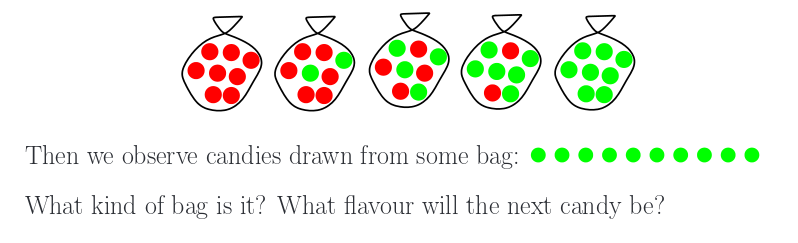
\includegraphics[scale=0.46]{candyEg.png}
    \end{center}
\end{frame}

\begin{frame}{Conditional Probability}
    \begin{itemize}
        \item $X, A =\langle A_1, A_2, \ldots, A_d \rangle$: Input feature vector
        \item $Y, C$: Class value to predict
        \item $P(C|A)$ vs $P(A|C)$ \pause
        \item Key terms
        \begin{itemize}
            \item $P(A), P(C)$: Prior probability
            \item $P(A|C)$: Class conditional probability or likelihood (from training data)
            \item $P(C|A)$: Posterior probability
        \end{itemize}
    \end{itemize}
\end{frame}

\begin{frame}{Likelihood vs Posterior}
    \begin{itemize}
        \item $P(A|C)$: Likelihood, $P(C|A)$: Posterior
        \item Examples:
        \begin{itemize}
            \item P(Viagra$|$Spam) and P(Spam$|$Viagra): \pause Likelihood, Posterior
            \item P(High temperature$|$Flu) and P(Flu$|$High Temperature): \pause Likelihood, Posterior
            \item P(Fever, Headache, Cough$|$Flu) and P(Flu$|$Fever, Headache, Cough)
            \item P(Viagra, Nigeria, Lottery$|$Spam) and P(Spam$|$Viagra, Nigeria, Lottery)
        \end{itemize}
    \end{itemize}
\end{frame}

\begin{frame}{Bayes' Theorem}
    \begin{itemize}
        \item Training data gives us likelihood and prior
        \item Prediction requires Posterior
        \item Bayes rule allows us to do statistical inference
        \item $P(C|A) = \frac{P(A|C) P(C)}{P(A)}$
        \item $P(C|A) \propto P(A|C) P(C)$
        \item Posterior $\propto$ Likelihood $\times$ Prior
    \end{itemize}
\end{frame}


\begin{frame}{Bayes Decision Rule}
    \begin{itemize}
        \item ``When you hear hoofbeats, think of horses not zebras''
        \item When predicting, assign the class with highest posterior probability
        \item To categorize email:
        \begin{itemize}
            \item Compute P(spam$|$email) and P(not spam$|$email)
            \item If P(spam$|$email) $>$ P(not spam$|$email), decide email as spam. Else as not-spam
        \end{itemize}
    \end{itemize}
\end{frame}


\section{Bayesian Classifiers}
\begin{frame}{} 
    \begin{center}
        \thblue{Bayesian Classifiers}
    \end{center}
\end{frame}

\begin{frame}{Bayes Classifier}
    \begin{center}
        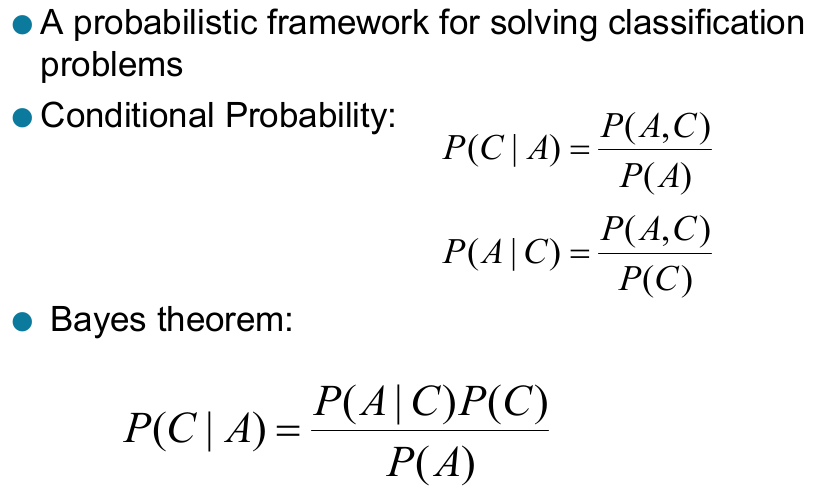
\includegraphics[scale=0.4]{bayesClassifier1.png}
    \end{center}
\end{frame}
\begin{frame}{Example of Bayes Theorem}
    \begin{center}
        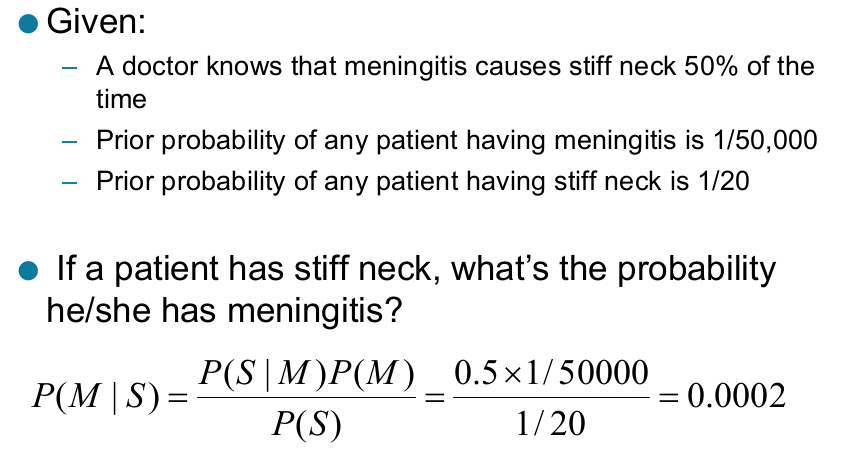
\includegraphics[scale=0.4]{bayesClassifier2.png}
    \end{center}
\end{frame}
\begin{frame}{Bayesian Classifiers}
    \begin{center}
        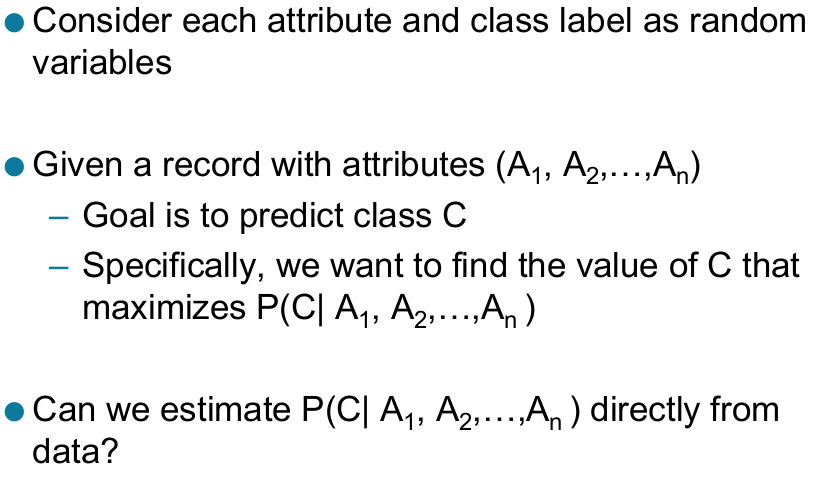
\includegraphics[scale=0.4]{bayesClassifier3.png}
    \end{center}
\end{frame}
\begin{frame}{Bayesian Classifiers}
    \begin{center}
        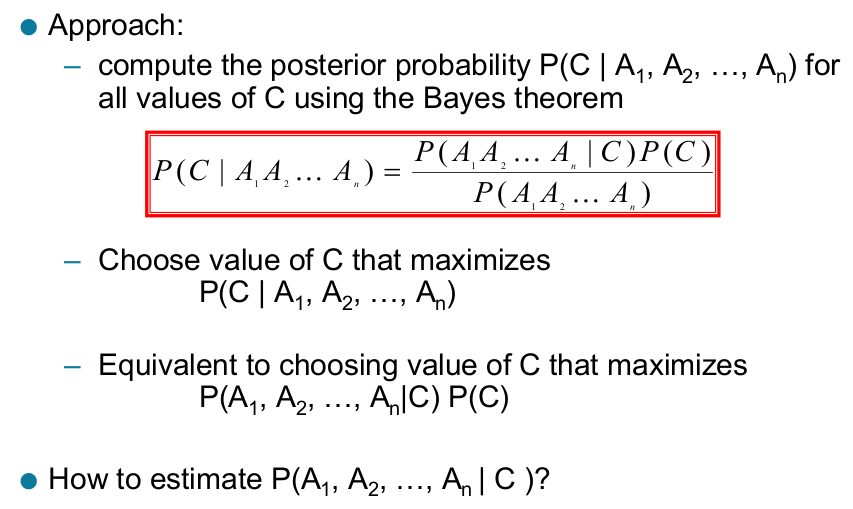
\includegraphics[scale=0.4]{bayesClassifier4.png}
    \end{center}
\end{frame}
\begin{frame}{Naive Bayes Classifier}
    \begin{center}
        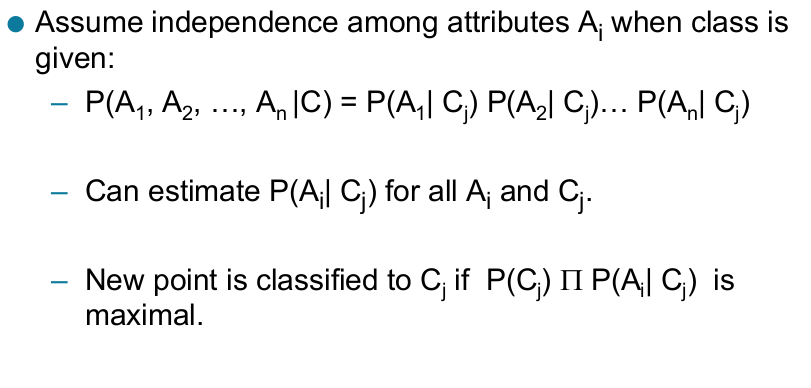
\includegraphics[scale=0.4]{bayesClassifier5.png}
    \end{center}
\end{frame}
\begin{frame}{How to Estimate Probabilities from Data?}
    \begin{center}
        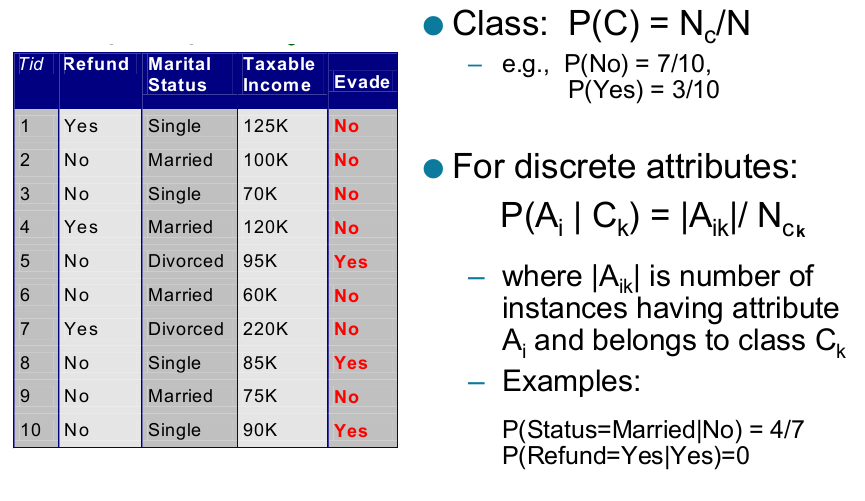
\includegraphics[scale=0.4]{bayesClassifier6.png}
    \end{center}
\end{frame}
\begin{frame}{How to Estimate Probabilities from Data?}
    \begin{center}
        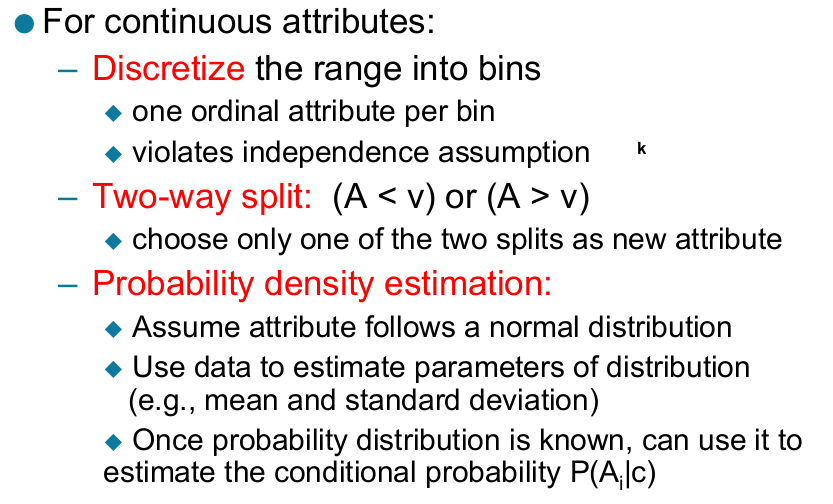
\includegraphics[scale=0.4]{bayesClassifier7.png}
    \end{center}
\end{frame}
\begin{frame}{How to Estimate Probabilities from Data?}
    \begin{center}
        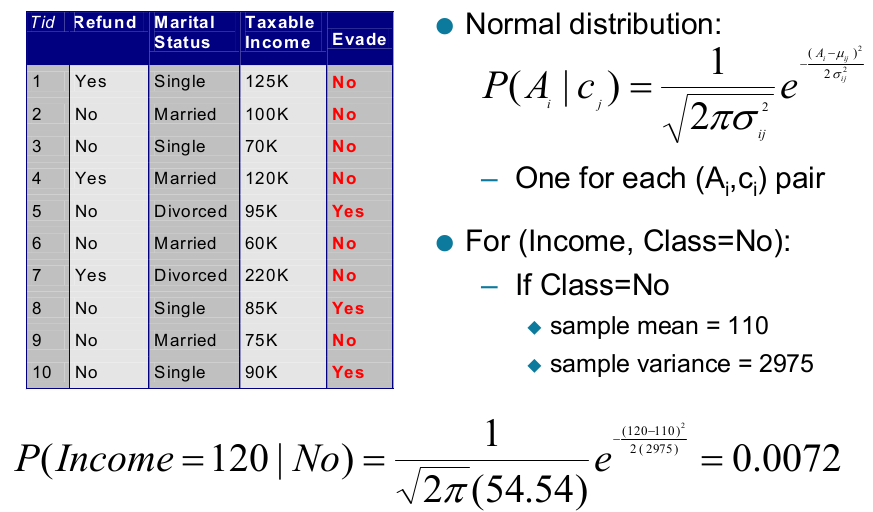
\includegraphics[scale=0.36]{bayesClassifier8.png}
    \end{center}
\end{frame}
\begin{frame}{Example of Naive Bayes Classifier}
    \begin{center}
        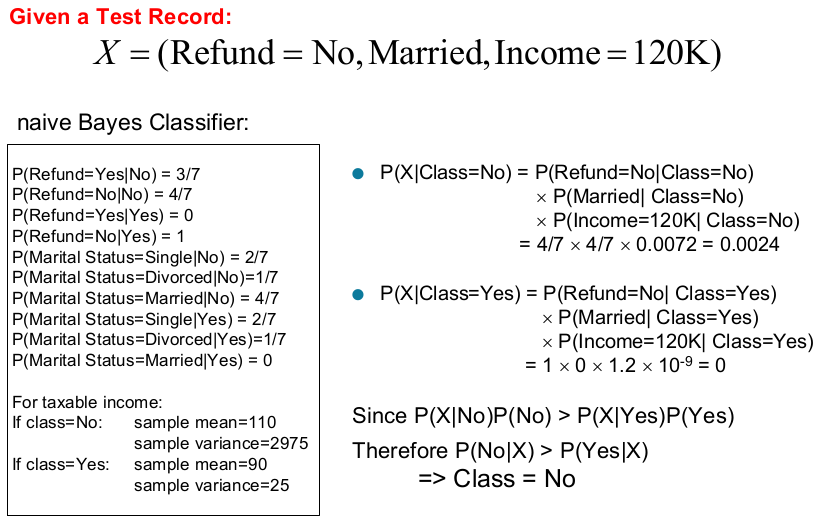
\includegraphics[scale=0.4]{bayesClassifier9.png}
    \end{center}
\end{frame}
\begin{frame}{Naive Bayes Classifier}
    \begin{center}
        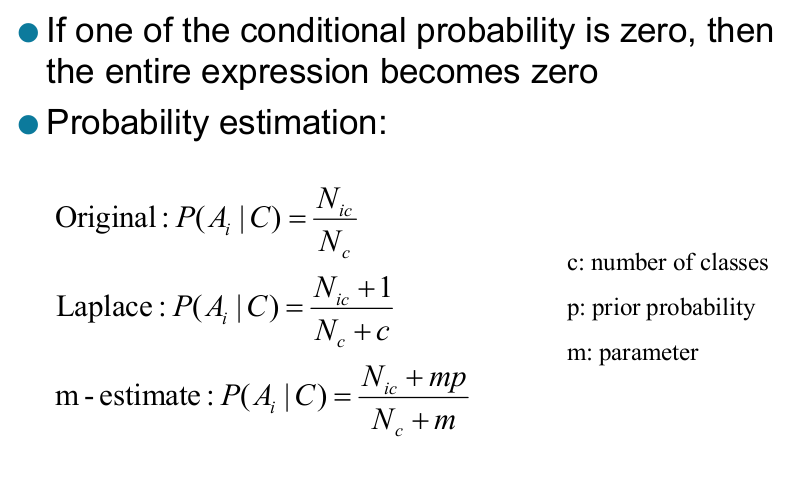
\includegraphics[scale=0.4]{bayesClassifier10.png}
    \end{center}
\end{frame}
\begin{frame}{Example of Naive Bayes Classifier}
    \begin{center}
        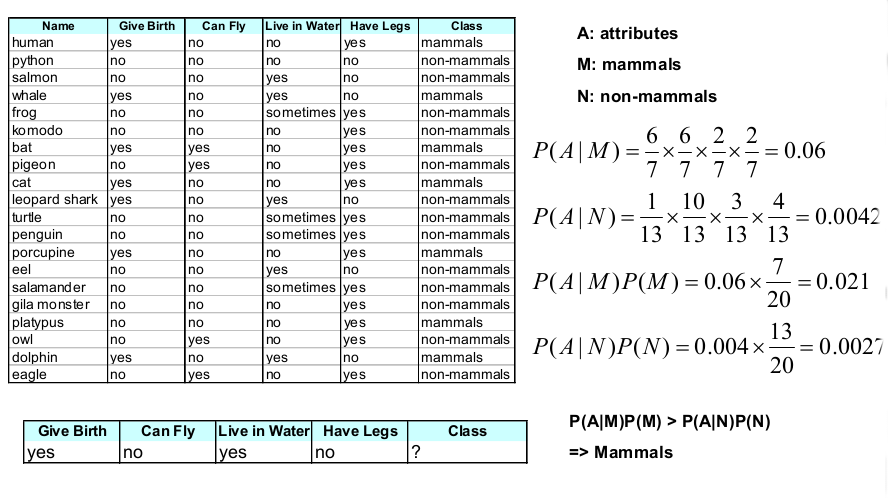
\includegraphics[scale=0.36]{bayesClassifier11.png}
    \end{center}
\end{frame}
\begin{frame}{Naive Bayes Classifier Summary}
    \begin{center}
        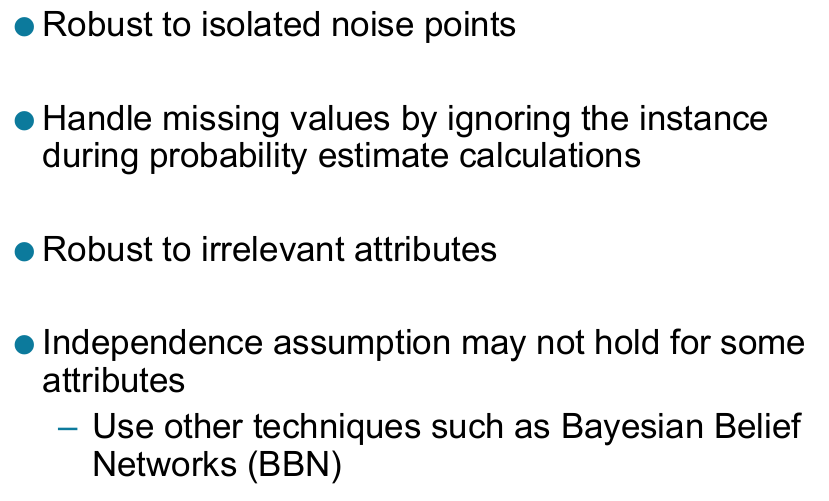
\includegraphics[scale=0.32]{bayesClassifier12.png}
    \end{center}
\end{frame}



\section{Support Vector Machines}
\begin{frame}{} 
    \begin{center}
        \thblue{Support Vector Machines}
    \end{center}
\end{frame}

\begin{frame}{HyperPlane}
    \begin{center}
        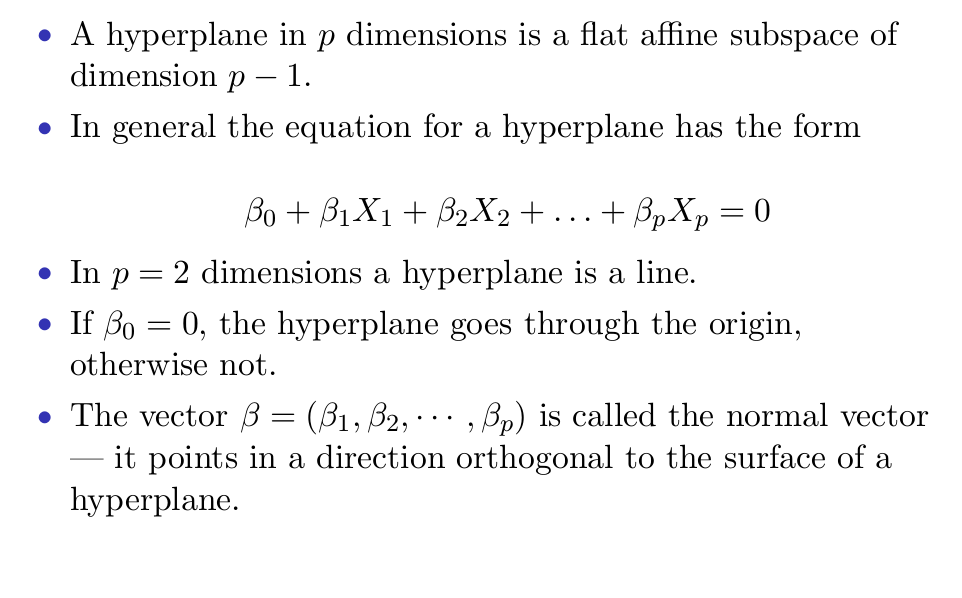
\includegraphics[scale=0.32]{hyerplane1.png}
    \end{center}
\end{frame}
\begin{frame}{HyperPlane in 2D}
    \begin{center}
        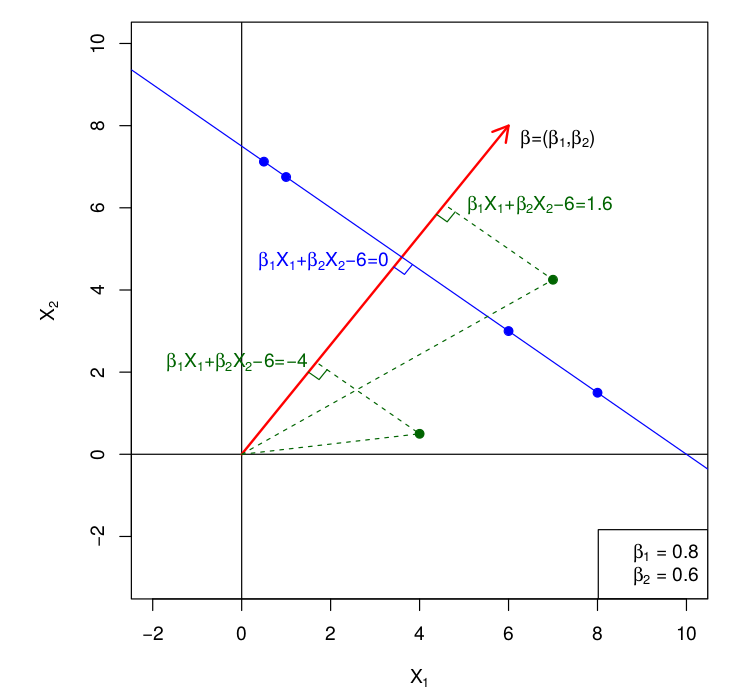
\includegraphics[scale=0.32]{hyerplane2.png}
    \end{center}
\end{frame}
\begin{frame}{Support Vector Machines}
    \begin{center}
        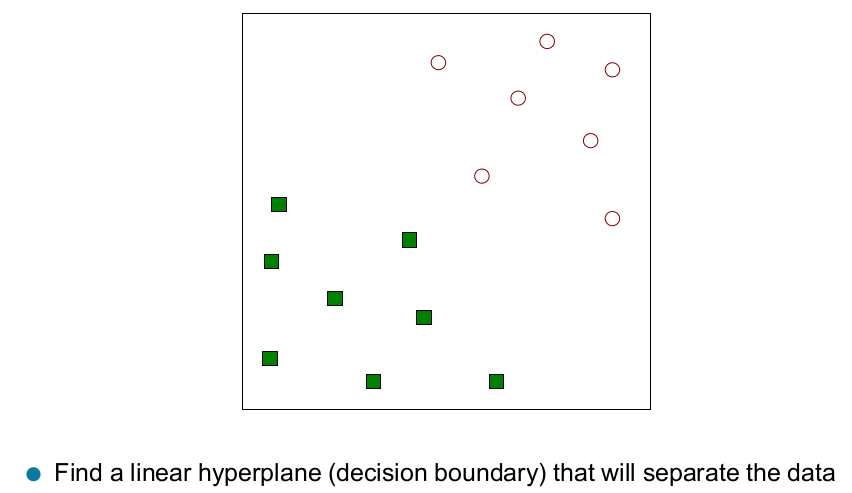
\includegraphics[scale=0.32]{svm1.png}
    \end{center}
\end{frame}
\begin{frame}{Support Vector Machines}
    \begin{center}
        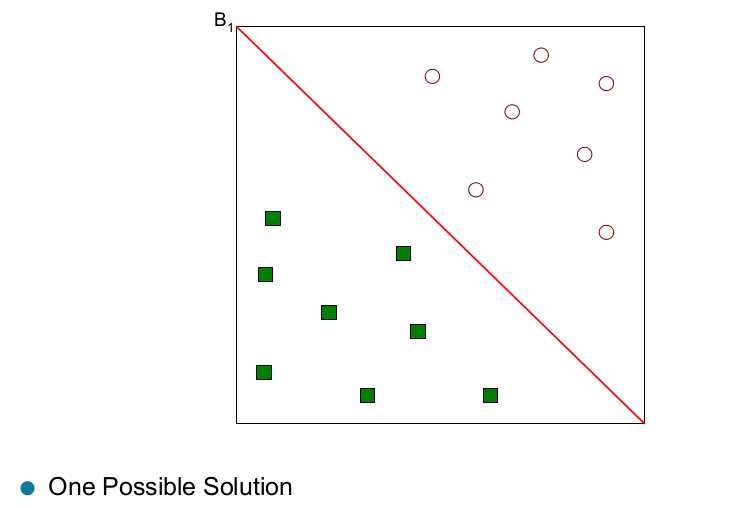
\includegraphics[scale=0.32]{svm2.png}
    \end{center}
\end{frame}
\begin{frame}{Support Vector Machines}
    \begin{center}
        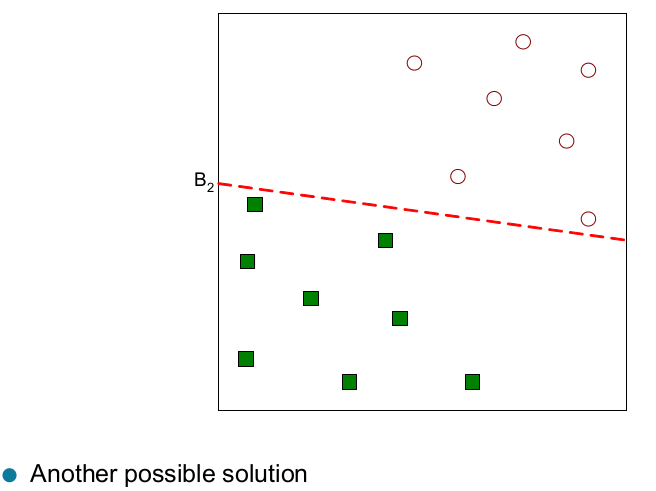
\includegraphics[scale=0.32]{svm3.png}
    \end{center}
\end{frame}
\begin{frame}{Support Vector Machines}
    \begin{center}
        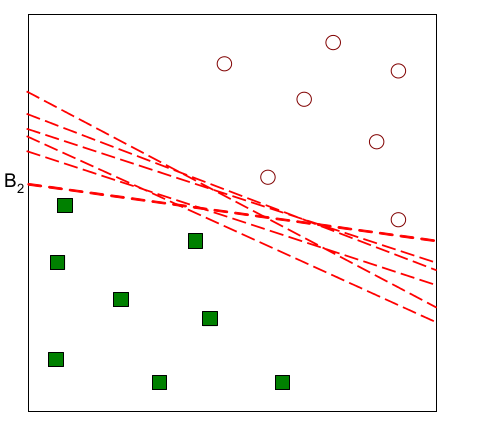
\includegraphics[scale=0.32]{svm4.png}
    \end{center}
\end{frame}
\begin{frame}{Support Vector Machines}
    \begin{center}
        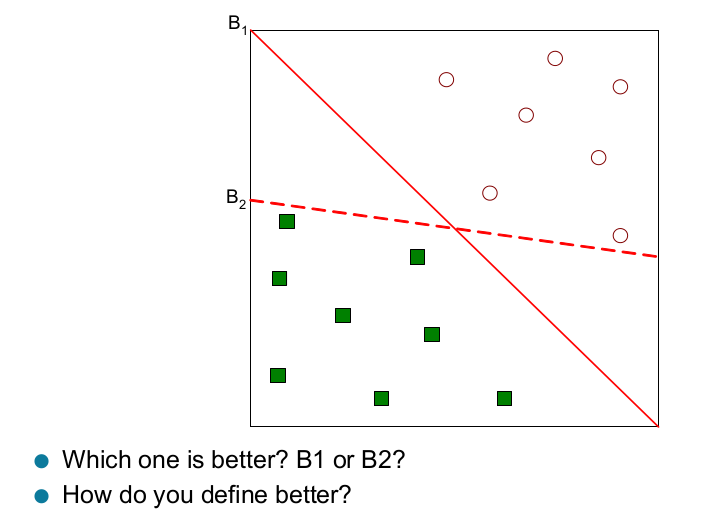
\includegraphics[scale=0.32]{svm5.png}
    \end{center}
\end{frame}
\begin{frame}{Support Vector Machines}
    \begin{center}
        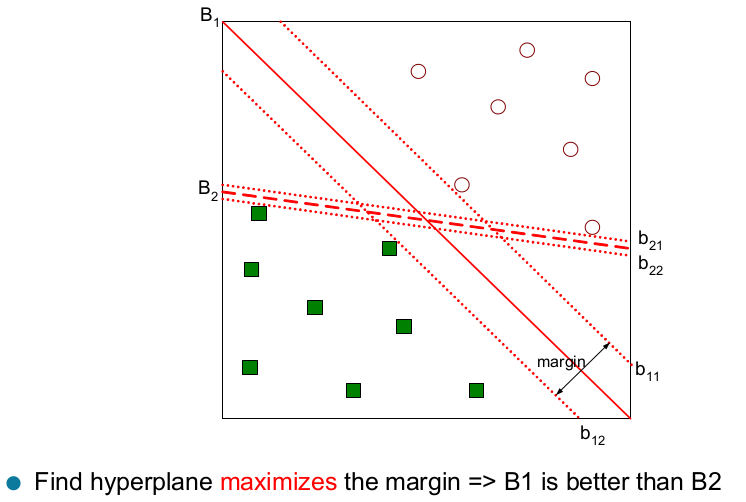
\includegraphics[scale=0.32]{svm6.png}
    \end{center}
\end{frame}
\begin{frame}{Support Vector Machines}
    \begin{center}
        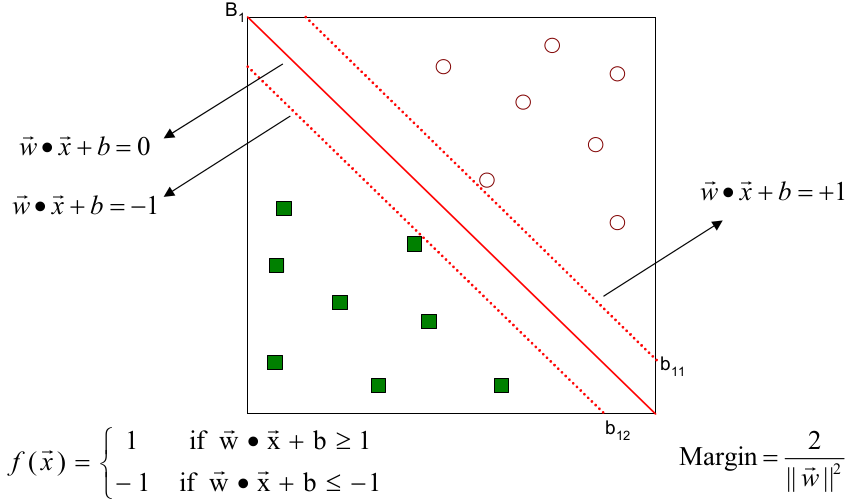
\includegraphics[scale=0.32]{svm7.png}
    \end{center}
\end{frame}
\begin{frame}{Support Vector Machines}
    \begin{center}
        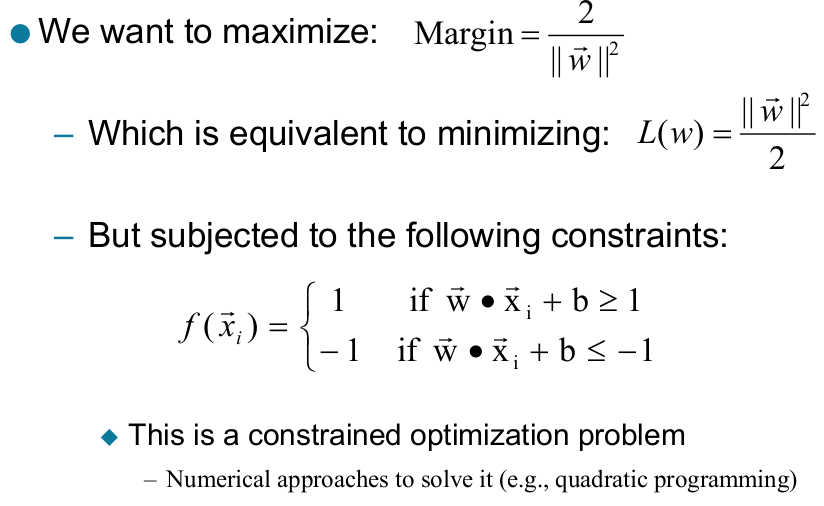
\includegraphics[scale=0.32]{svm8.png}
    \end{center}
\end{frame}
\begin{frame}{Support Vector Machines}
    \begin{center}
        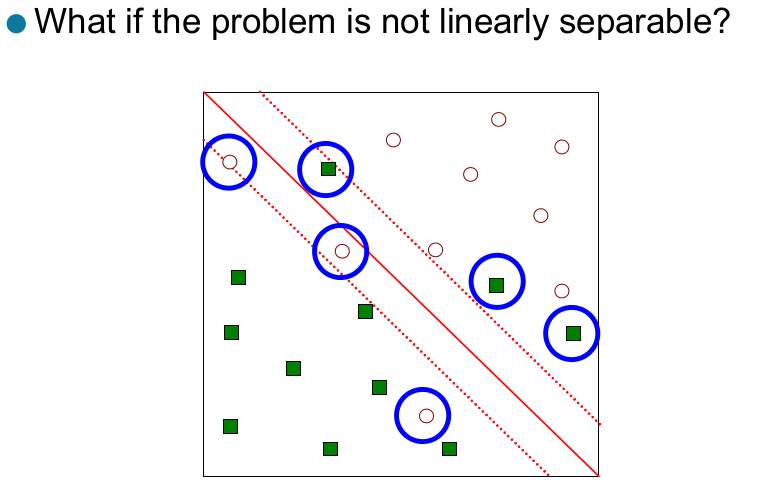
\includegraphics[scale=0.32]{svm9.png}
    \end{center}
\end{frame}
\begin{frame}{Support Vector Machines}
    \begin{center}
        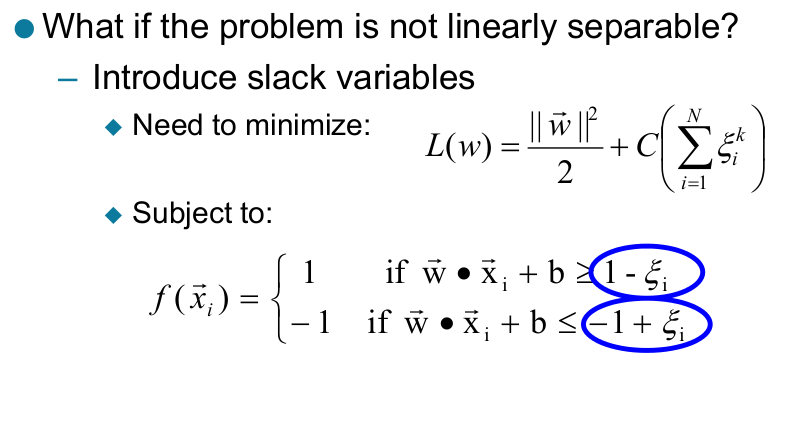
\includegraphics[scale=0.32]{svm10.png}
    \end{center}
\end{frame}
\begin{frame}{Nonlinear Support Vector Machines}
    \begin{center}
        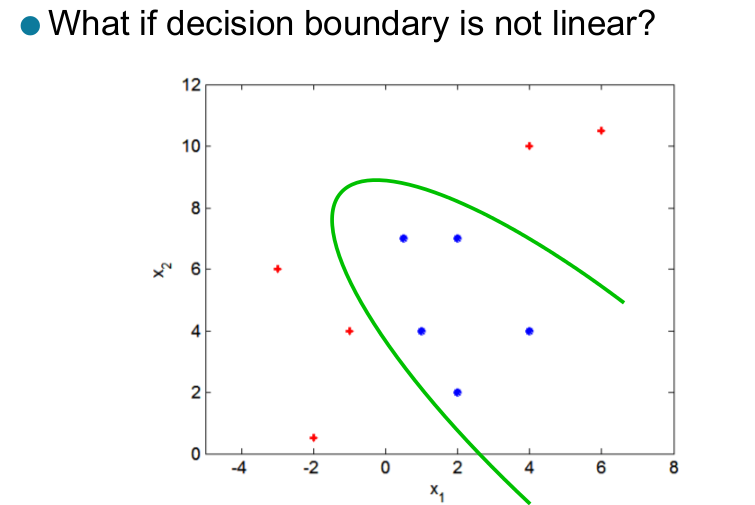
\includegraphics[scale=0.32]{svm11.png}
    \end{center}
\end{frame}
\begin{frame}{Nonlinear Support Vector Machines}
    \begin{center}
        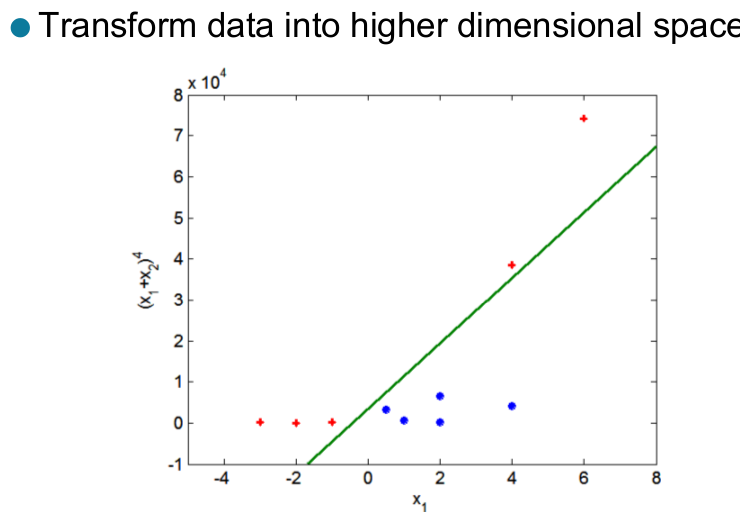
\includegraphics[scale=0.32]{svm12.png}
    \end{center}
\end{frame}
\begin{frame}{Kernels}
    \begin{center}
        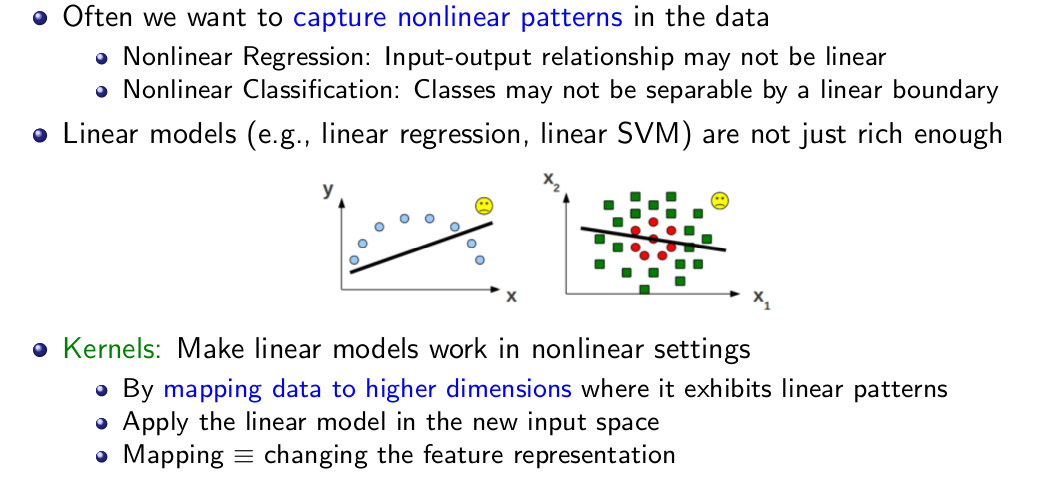
\includegraphics[scale=0.32]{kernels1.png}
    \end{center}
\end{frame}
\begin{frame}{Classifying non-linearly separable data}
    \begin{center}
        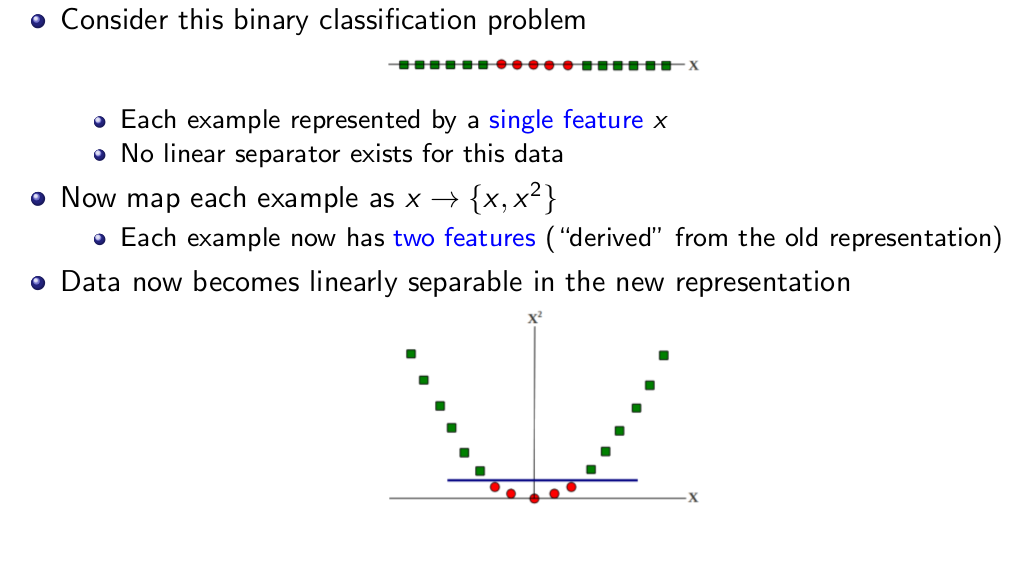
\includegraphics[scale=0.32]{kernels2.png}
    \end{center}
\end{frame}
\begin{frame}{Classifying non-linearly separable data}
    \begin{center}
        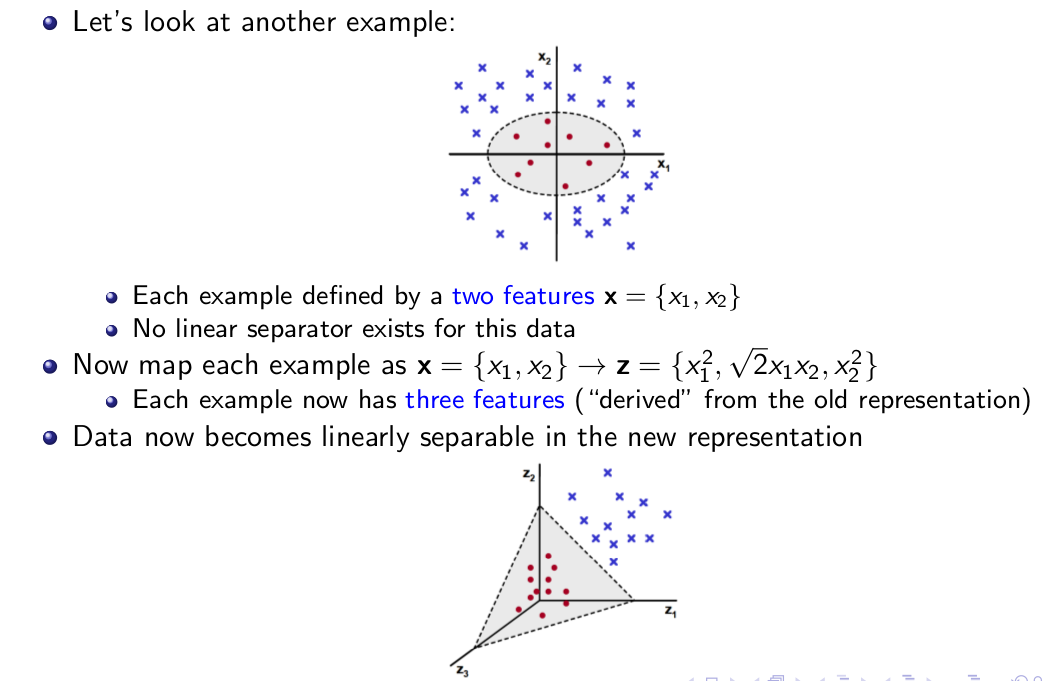
\includegraphics[scale=0.32]{kernels3.png}
    \end{center}
\end{frame}
\begin{frame}{Feature Mapping}
    \begin{center}
        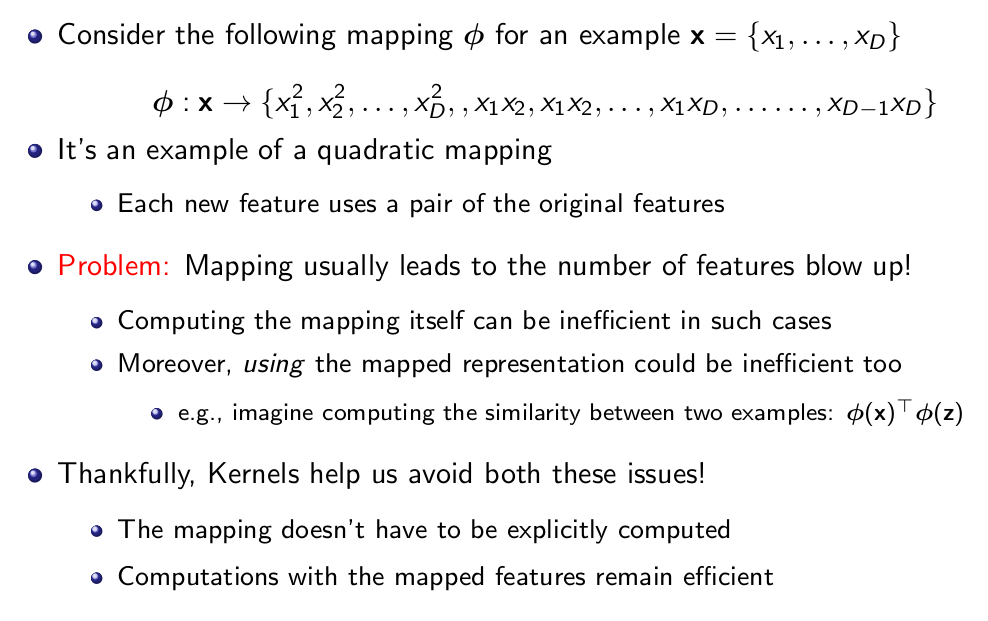
\includegraphics[scale=0.32]{kernels4.png}
    \end{center}
\end{frame}
\begin{frame}{Kernels as High Dimensional Feature Mapping}
    \begin{center}
        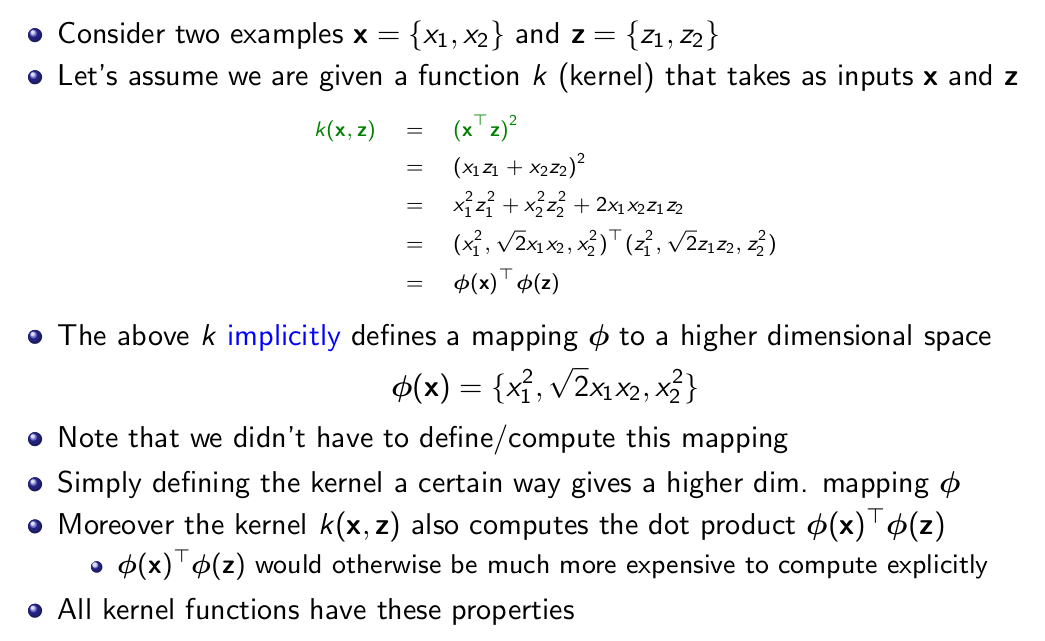
\includegraphics[scale=0.32]{kernels5.png}
    \end{center}
\end{frame}
\begin{frame}{Kernels: Formally Defined}
    \begin{center}
        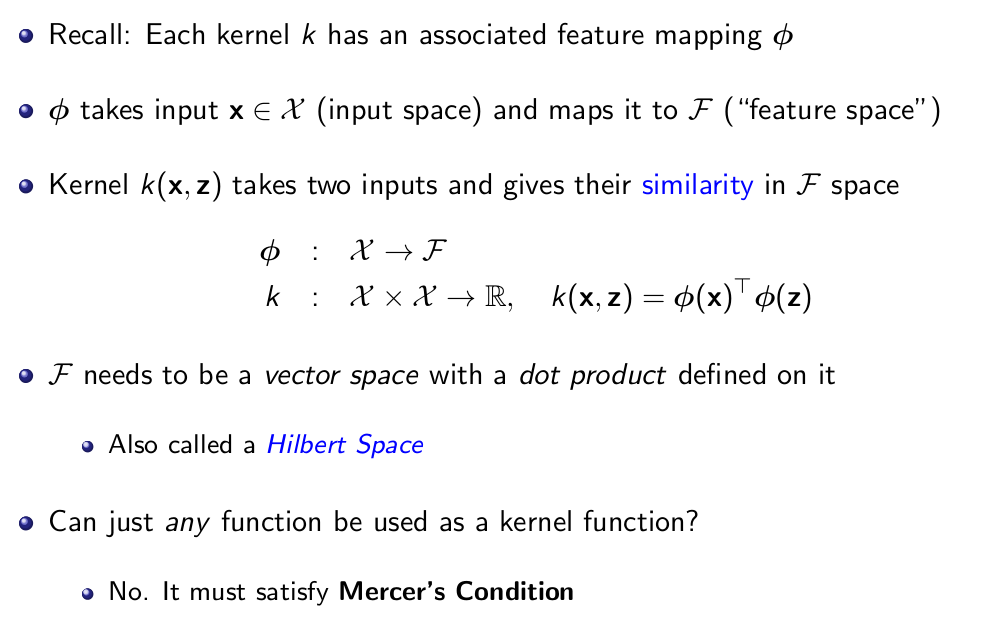
\includegraphics[scale=0.32]{kernels6.png}
    \end{center}
\end{frame}
\begin{frame}{Popular Kernels}
    \begin{center}
        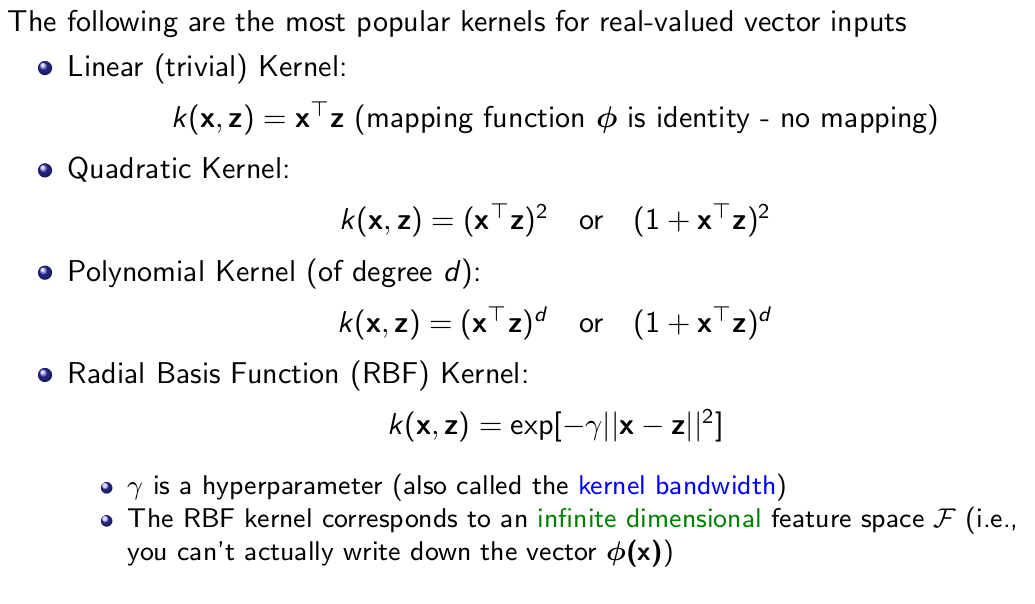
\includegraphics[scale=0.32]{kernels7.png}
    \end{center}
\end{frame}
\begin{frame}{Using Kernels}
    \begin{center}
        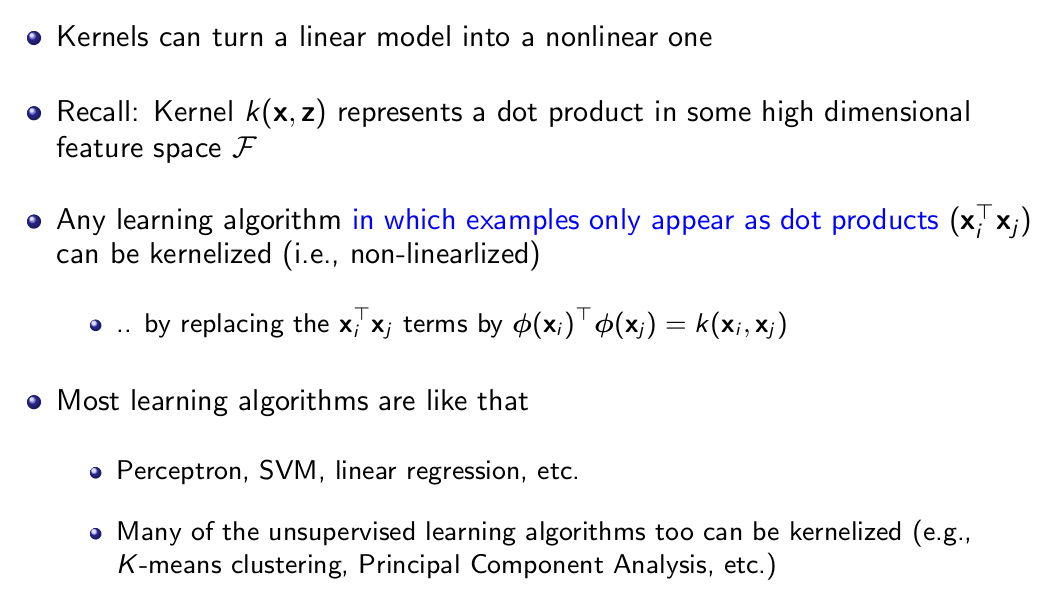
\includegraphics[scale=0.32]{kernels8.png}
    \end{center}
\end{frame}


\section{Summary}
\begin{frame}{Summary}

\tblue{Major Concepts:}
\begin{itemize}
    \item Probabilistic interpretation of Classification
    \item Bayesian Classifiers
    \item Naive Bayes Classifier
    \item Support Vector Machines (SVM)
    \item Kernels
\end{itemize}
\end{frame}

\begin{frame}{Slide Material References}
\begin{itemize}
    \item Slides from TSK Book, Chapter 5 
    \item Slides from Piyush Rai 
    \item See also the footnotes
\end{itemize}
\end{frame}


\end{document}

